\chapter{System Overview}

\begin{figure}[t]
  \centering
  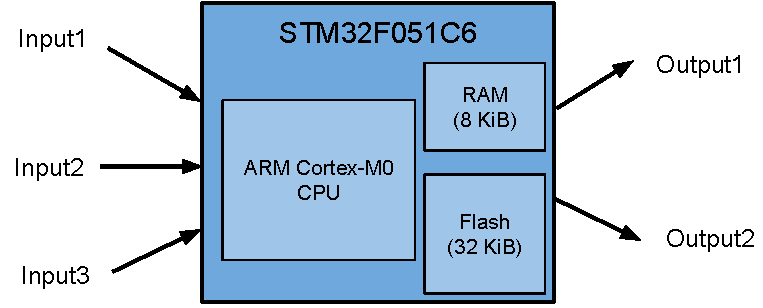
\includegraphics[width=0.9\textwidth]{./week1/programmers_model_v0.pdf}
  \caption{The most simplified view of the internals of the STM32F051}
  \label{fig:prog_mod_v0}
\end{figure}

\section{What is a Microcontroller?}
The microcontroller can be understood by comparing it to something you are already very familiar with: the computer. Both a microcontroller and a computer can be modeled as a black box which takes in data and instructions, performs processing, and provides output.
In order to do this, a micro has some of the same internals as a computer, shown graphically in \autoref{fig:prog_mod_v0} and discussed now:
\begin{itemize}
  \item CPU: The section of the microcontroller which does the processing. It executes instructions which allows it to do arithmetic and logic operations, amongst other forms of operations.
  \item  Volatile memory (RAM:) This is general purpose memory. It can be used for storing whatever you want to store in it. Typically it stores variables which are created or changed during the course of execution of a program.
  \item Non-volatile memory (Flash): This non-volatile memory is used to store any date which must not be lost when the power to the micro is removed. Typically this would include the program code and any constants or initial values of data.
  \item Ports: Interfaces for data to move in and out of the micro. This allow it to communicate with the outside world. 
\end{itemize} 
These resources are typically orders of magnitude smaller or a micro than on a conventional computer. A micro makes up for this lack of resources with a small size, low power and low cost. A comparison of the characteristics can be seen in \autoref{table:specs_comp}.
A computer is typically defined as a multi-purpose, flexible unit able to do computation. A microcontroller on the other hand typically is hard-coded to do one specific job.\\

\begin{table}
\begin{tabu}{ >{\textbf}c | c  c  c  c  c  c }
  & \textbf{CPU} & \textbf{RAM} & \textbf{Non-volatile} & \textbf{Power} & \textbf{Size/Mass} & \textbf{Cost} \\
  \hline
  \textbf{Computer} & Dual, 3 GHz & 4 GiB & 500 GB & 100 W & Large & R 3000 \\
  \textbf{Micro} & 48 MHz & 8 KiB & 32 KiB & 50 mW & Small & R 15 \\
\end{tabu}
\caption{Comparison of specs of entry level computer to STM32F051C6.}
\label{table:specs_comp}
\end{table}

The terms \textit{microcontroller} and \textit{microprocessor} are different and should not be used interchangably. A microprocessor is an IC which is able to perform computation, but requires external memory and perihperals to function. A microcontroller has the memory and perihperals built into it, allowing it to be fully independant. Furthermore, the interface in and out of a microprocessor is mainly just an address and data bus. In a microcontroller, these busses are internal to the device. The interfaces in and out of a microcontroller are configurable to be a wide variety of communication standards.\\

The micro we will be using is the STM32F051C6. It is manufactured by ST Microelectronics, but has an ARM Cortex-M0 CPU. ARM designed the CPU (specified how the transistors connect together). ST then takes this CPU design, adds it to their design for all of the other bits of the micro (flash, RAM, ports and much much more) and then produces the chip.

\subsection{Development board block diagram}
The development board consists of modules which connect to the microcontroller. Most of these modules are optional in that they are not required for the microcontroller to run. We will develop code later in the course to interface with some of these modules. Those which are not optional are the voltage regulator and the debugger.
Following is a breif discussion of the purpose of each of the dev board modules (peripherals).

\begin{figure}
  \centering
  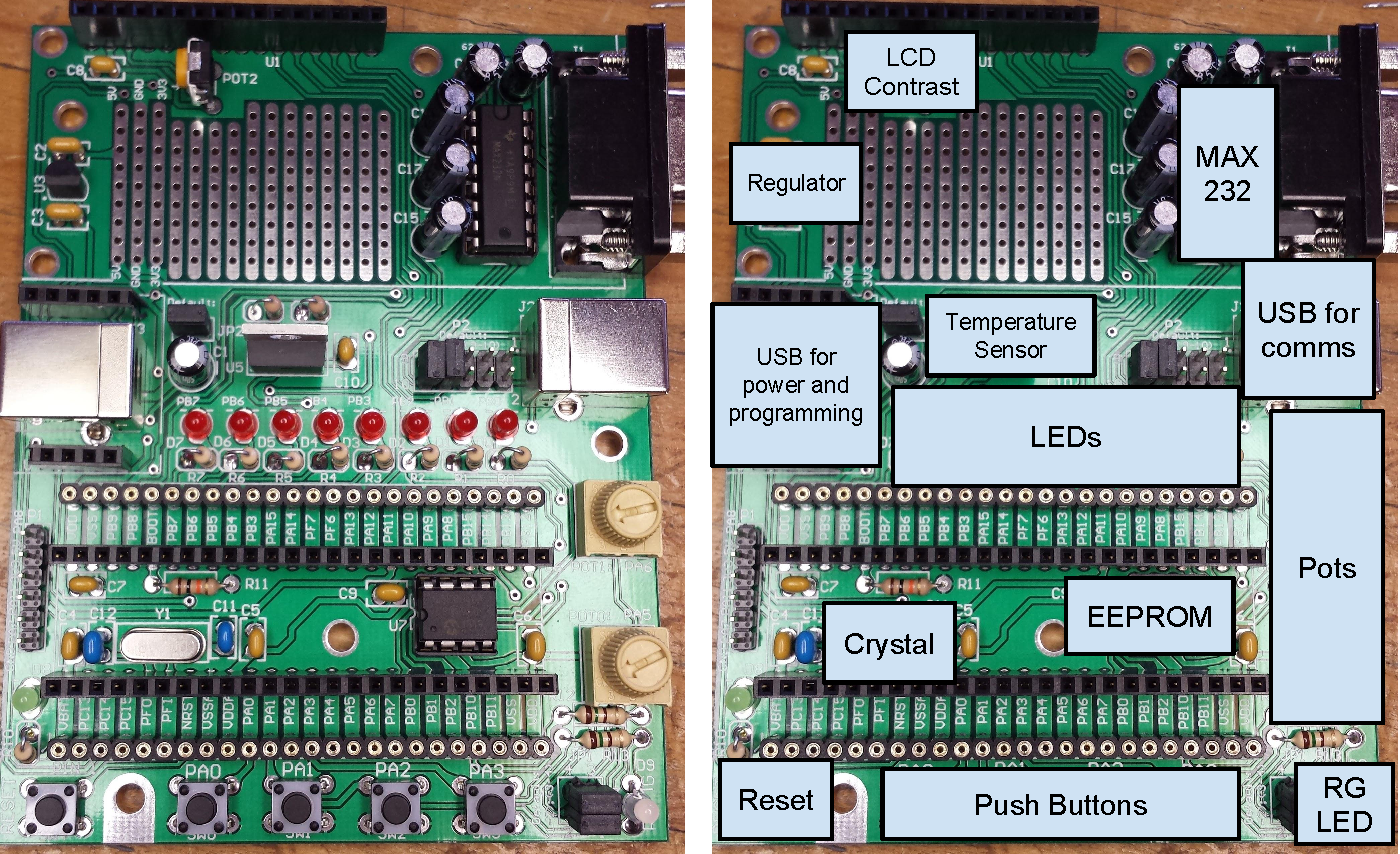
\includegraphics[width=\textwidth]{./week1/dev_board_unplugged.pdf}\\
  \vspace{3mm}
  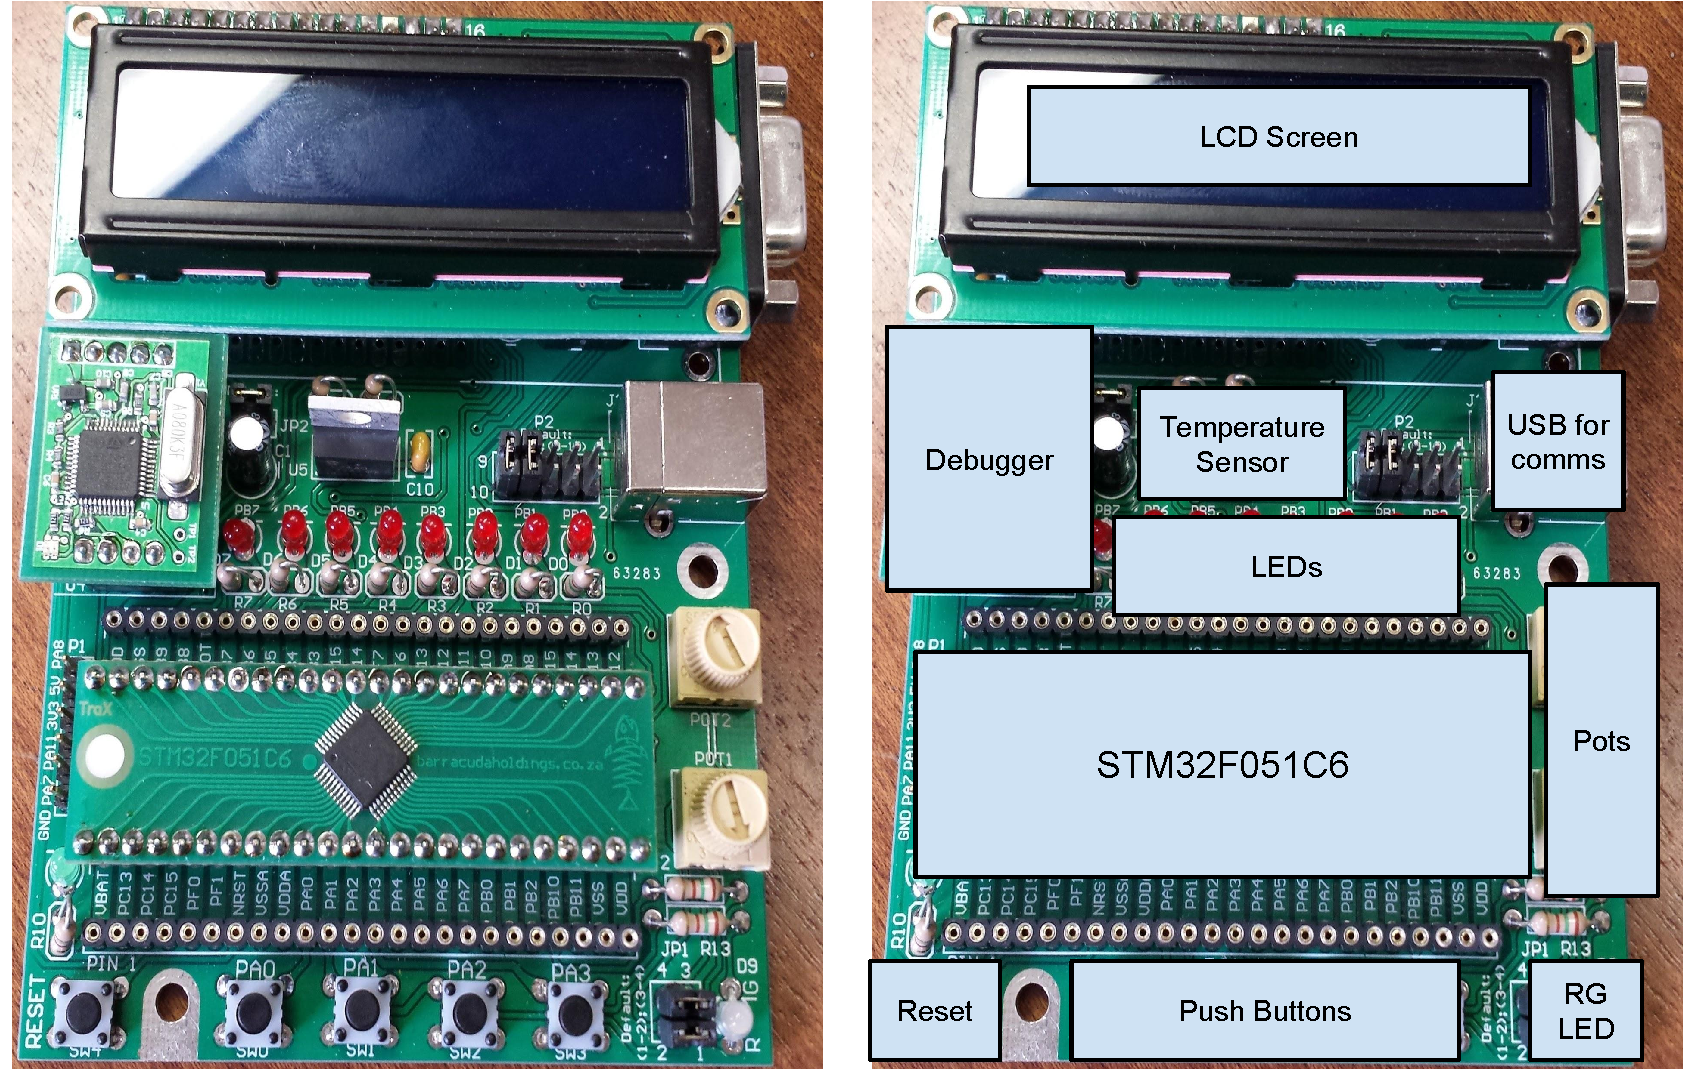
\includegraphics[width=\textwidth]{./week1/dev_board_plugged_in.pdf}
  \caption{Modules on the dev board as seen when top boards unplugged or plugged in}
\end{figure}

\begin{itemize}
  \item STM32F051C6: This is the target microcontroller. It is connected to everything else on the board and it is where the code which we develop will execute. 
  \item The debugger is essentially another microcontroller which is able to pass information between a computer and a target microcontroller. The interface to the computer is a USB connection, and the interface to the target is a protocol called Serial Wire Debug (SWD) which is similar to JTAG. 
  \item Regulator: A MCP1702-33/T0 chip. This converts the 5 V provided by the USB port into 3.3 V suitable for running most of the circuitry on the board. 
  \item LEDs: One byte of LEDs, active high connected to the lower byte of port B.
  \item Push buttons: Active low push buttons connected to the lower nybble of port A.
  \item Pots: 2 x 10K (or there abouts) potentiometers connected to PA5 and PA6.
  \item LCD Screen: A 16x2 screen connected to the micro in 4-bit mode. Used to display text.
  \item LCD contrast pot: The output of this potentiometer connects to the contrast pin of the LCD screen, hence allowing contrast adjustment.
  \item MAX232: This chips translates between TTL or CMOST logic level UART traffic and bi-polar higher voltage RS-232 traffic. Used for industrial communications links.
  \item USB for comms: The header allows intercapting of the UART traffic before it gets to the MAX232 and convertin it to USB traffic through a small board which plugs into that header. When this facility is not being used, the jumpers on the header should be placed to allow the UART traffic to make its way to the MAX232.
  \item Temperature sensor: A TC74-A0 $I^2C$ temperature sensor.
  \item Crystal: 8 MHz quartz oscillator with 10 pF caps for removing high frequency harmonics. 
  \item EEPROM: A 25LC640A 64Kb Electronically Erasable and Programmable Read Only Memory SPI chip.
  \item RG LED: Common cathod Red/Green LED
\end{itemize}

    For now, we will forget about all of the other modules on the dev board and consider our system to be a computer talking to a debugger talking to a target micro, as shown in \autoref{fig:debugger_to_micro}. 

\begin{figure}[t]
  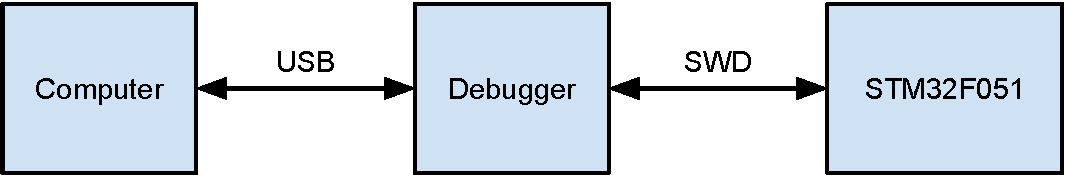
\includegraphics[width=\textwidth]{./week1/debugger_to_micro.pdf}
  \caption{Highly simpified diagram showing how micro and computer communicate}
  \label{fig:debugger_to_micro}
\end{figure}

This is the most basic system which must be understood to allow us to load code onto the target microcontroller.



\chapter{The ARM Cortex-M0}

\subsection{Programmer's Model of the CPU}
\begin{figure}[t]
  \centering
  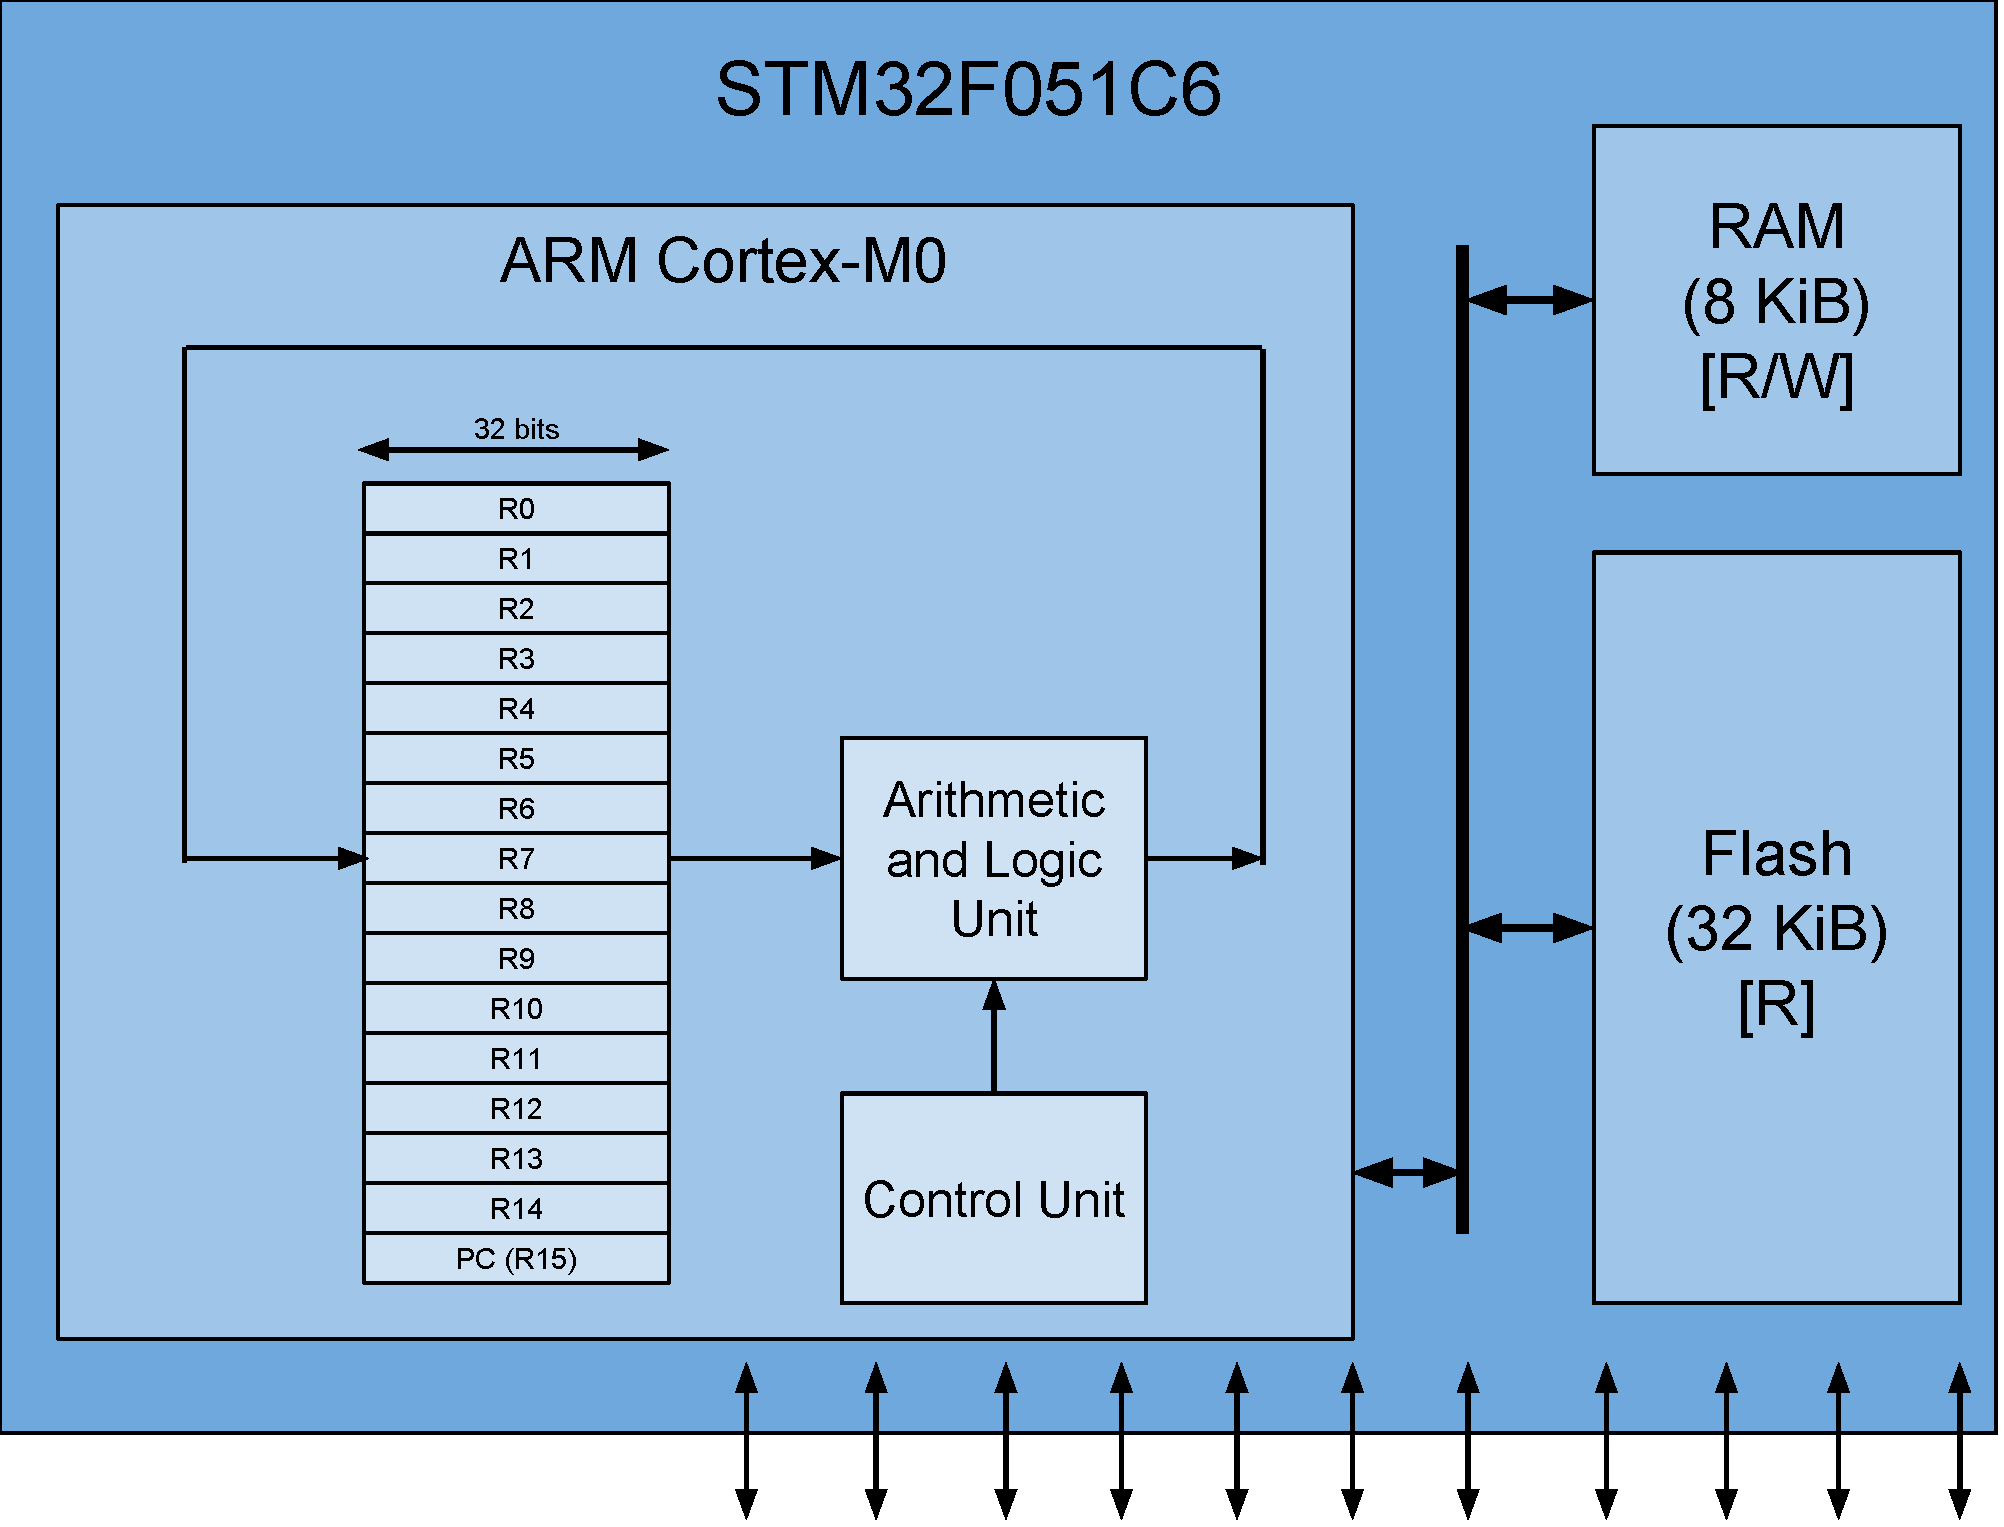
\includegraphics[width=0.9\textwidth]{./week1/programmers_model_v1.pdf}
  \caption{A view of the internals of the STM32F051 with the ARM Cortex-M0 expanded}
  \label{fig:prog_mod_v1}
\end{figure}
In \autoref{fig:prog_mod_v0} we saw that the basic components were a CPU, flash, RAM and ports. This chapter seeks to explore the CPU in some detail. The expanded view of the CPU which will now be discussed can be seen in \autoref{fig:prog_mod_v1}. This simple model of a CPU is a set of CPU registers, an Arithmetic and Logic Unit (ALU) and a control Unit. The CPU registers are blocks of storage each 32 bits wide which the CPU has the ability to operate on. Only data which is inside a CPU register can be operated on by the CPU. The ARM Cortex-M0 has 16 such registers. 

The ALU is that performs the operations on the registers. It can take data from registers as inputs, do very basic processing and store the result in CPU registers. 

The control unit manages execution by telling the ALU what to do. Together, the registers, ALU and control are able to execute instructions. 
Examples of instructions which the CPU is able to execute:
\begin{enumerate}
  \item adding the contents of R0 and R1 and storing the result in R6
  \item copying the contents of R3 into R0
  \item doing a logical XOR of the contents of R3 with the contents of R4 and storing the result in R3
  \item moving the number 42 into R5
\end{enumerate}

ARM defines datatypes for a 32 bit CPU as follows:
\begin{itemize}
  \item byte: 8 bits
  \item halfword: 16 bits
  \item word: 32 bits
  \item doubleword: 64 bits
\end{itemize}

\section{CPU Architecture}
This section will explore some CPU architectures and compare them to the architecture of the Cortex-M0.

The Cortex-M0 makes use of a Von Neumann architecture. This means that there is a single bus which connects all perihperals inside the microcontroller. The implication of this is that the CPU cannot fetch an instruction from flash at the same time as it moves data in or out of RAM. This limitation allows for a much simpler architecture.

Other microcontrollers (even others in the Cortex-M series like the Cortex-M3) follow a Harvard architecture, meaning that there are seperate busses used for fetching instructions and moving data around. This allows faster execution as instructions can be fetched at the same time as data is loaded or stored. However, it necessitates greater complexity and more transistors. 

\chapter{Memory Model}
\begin{figure}
  \centering
  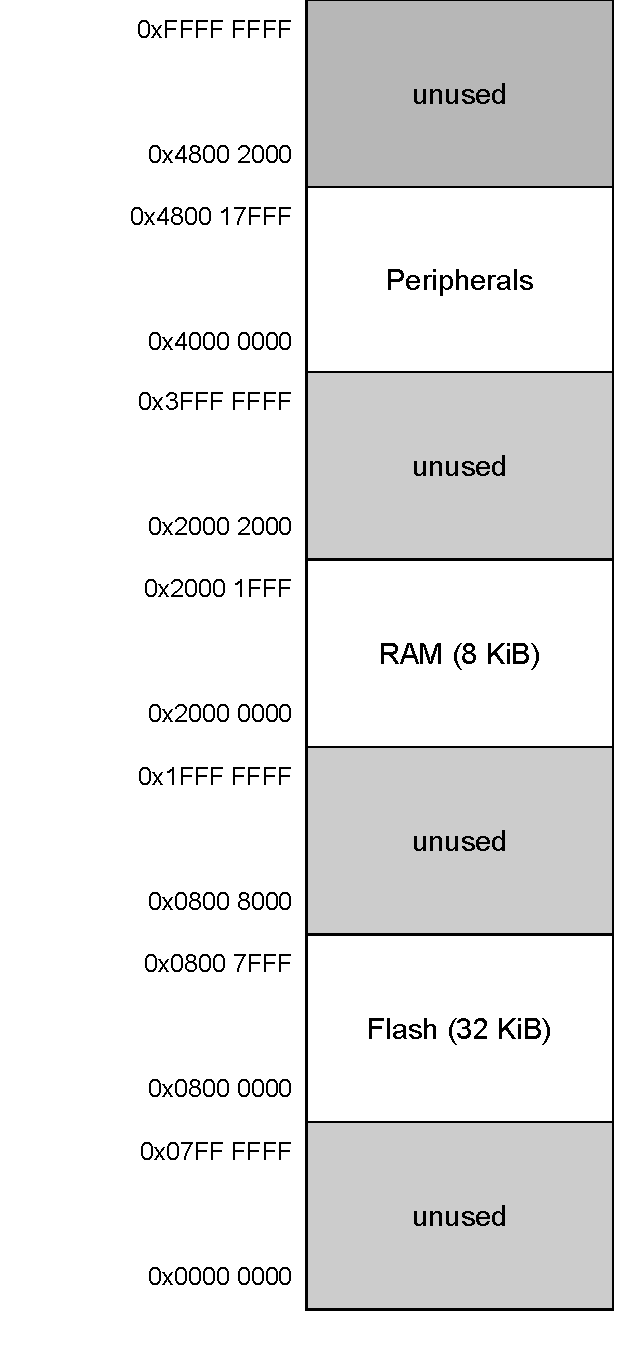
\includegraphics[width=0.6\textwidth]{./week1/memory_model_v0.pdf}
  \caption{Simplified STM32F051C6 memory map. Note how all addresses are 32 bits. The blocks are very much not to scale. Source: datasheet, Figure 9}
\end{figure}
The memory of a device can be though of as a very long row of post boxes along a street. Each post box has an address, and each post box can have data put into it or taken out. The amount of data that each post box can hold is 8 bits, or one byte. 
The address of each post box is 32 bits long, meaning that addresses range from 0 (0x00000000) to just over 4 billion (0xFFFFFFFF). In actual fact, the \emph{vast} majority of these addresses do not have a post box at them. These addresses are said to be unimplemented. 
Only very small sections of this address space are implemented and can actually be read from or written to.
The sections which we are interested in are flash, RAM and peripherals (more on these later). Flash and RAM are contiguous blocks of memory, with a start address and an end address. \\

Once our assembly code has been written and compiled to machine code, the computer which loads the code onto the micro has to be told what addresses to place the code at. The code should be placed starting at the beginning of flash. 

\subsection{Writing and compiling code}
In order to get the CPU to do some of what we've discussed above, it needs to have code loaded onto it to run. We write code in a language called assembly. Assembly is a human-readable language. A program is made up of a sequence of instruction; each instruction gets executed by the CPU. It's quite easy to see what each instruction does by reading the program.  The complete instruction set is located in the Programming Manual. You must be familiar with this document! Examples of instruction which carry out the tasks listed above are:
\begin{enumerate}
  \item \texttt{ADDS R6, R0, R1}
  \item \texttt{MOV R0, R3}
  \item \texttt{EORS R3, R3, R4}
  \item \texttt{MOVS R5, \#42}
\end{enumerate}
The CPU does not have the ability to understand our nice English words like \textit{ADD} or \textit{MOV}. The CPU only has the ability to understand binary data. Assembly code must be compiled to machine code. A machine code instruction is a binary string, 16 bits long consisting of the operation code (opcode) and the data which it must operate on (operand).
For example, assume that we wanted to ascertain the machine code representation of the instruction \texttt{ADDS R6, R0, R1}. An extact from the ARMv6-M Architecture Reference Manual is shown in \autoref{fig:adds_encoding} where Rd is the destination register and Rm and Rn are the source registers of the add. It can easily be seen that the instruction would compile to\texttt{ 0001100 001 000 110 = 0x1846}.
\begin{figure}
\centering
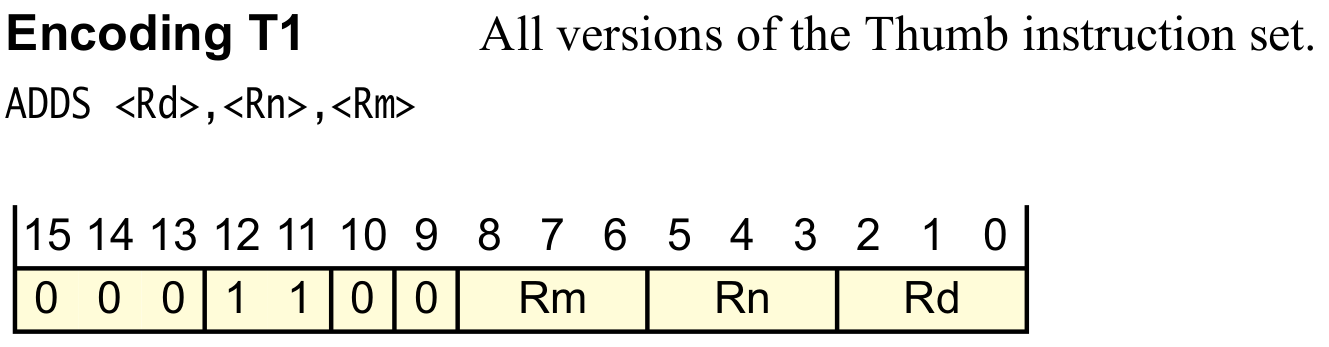
\includegraphics[width=0.7\textwidth]{./week1/adds_encoding}
\caption{An encoding of the ADDS instruction}
\label{fig:adds_encoding}
\end{figure}
The opcodes for each instruction are detailed in the ARMv6-M Architecture Reference Manual.
All of the instructions in the program are 16 bits long and are stored sequentially after one another in flash memory. 

\subsection{Instruction Sets}
An instruction set is the collection of all of the instructions which a processor can execute. 
The ARM Cortex-M0 uses the ARMv6-M architecture and this architecture supports the Thumb instruction set (as opposed to Thumb-2 or ARM). 
Thumb contains about \emph{XXX} instructions, each of which is 16 bits long. \\

Higher end ARM processors such as the Cortex-M3 or Cortex-M4 support the ARMv7-M architecture which allows multiple instruction sets to be supported by the processor. 
The ability to support multiple instruction sets requires \emph{interworking}. Interworking is the ability to specify to the CPU which instruction set to use. 
While our ARM Cortex-M0 only supports the Thumb instruction set, there is no need for interworking, yet the cabability has still been incorperated into the architecture to allow for compatability to other processors. 
This means that although our processor only supports one instruction set (Thumb), we have to explicity tell it that we are using that instruction set. 


\subsection{Executing Code}
Once the code has been loaded onto the microcontroller, it will execute one instruction after the next. 
CPU register R15 is reserved for keeping track of where the micro is in execution. It is known as the Program Counter (PC).
The PC always points to the instruction which is ABOUT to be executed. Hence, when your micro boots up, before it has executed anything, the PC will point to the first instruction to be executed.
By ``point to'' we mean that it holds the address of the instruction. 

As each instruction in the ARM Cortex-M0 instruction set it 16 bits (aka: half a word) long, ARM have implemented a rule that all instructions must be half word alligned. In other words, the address of the instruction must be divisible by 2 bytes. Legal addresses for instructions are hence, 0x02, 0x04, 0x06, 0x08 ... etc. 
This means that the least significant bit (bit 0) of the PC register is unused in specifcying the address of an instruction. 
Hence, it has been assigned another use. Specifically, to indicate the type of instruction which is being executed. 



\subsection{A basic model of the STM32F051}

\subsection{The ARM Cortex-M0}
The microcontroller which we will be using is the STM32F051C6. At the core of this micro is it's CPU, which is called the Cortex-M0 and is designed by Advanced RISC Machines (ARM).a]]

It's been said that the ARM Cortex-M0 is a 32-bit processor. For comparison, the procesor which we used in this course previously (MC9S08GT16A) was an 8-bit processor. Your personal computer probably has a 64-bit CPU. 16-bit CPUs are also quite common. So what exactly does it mean when we say that the processor is 32-bits? Essentially, the number of bits which a processor is said to be referes to the size of the data bus. In other words: the amount of data which the processor is able to move around internally or perform arithmetic and logic operations on. Hence, with a 32-bit processor, we can move 32 bits of data from one spot in memory to another in just once instruction. If you had a 8-bit processor, it would cost 4 instructions to move 32 bits of data around.  



\subsection{A Short History of ARM}
Acorn

\chapter{Perihperals}
Ports are typically controlled by a block of memory called perihperals. Unlike RAM which is general purpose, each register in the perihperals memory block has a specific, well defined purpose. Typically the purpose of these perihperal registes are for configuring the microcontroller to behave in a certain way or communicate with the outside world.
These CPU registers are different to the peripheral registers mentioned earlier for the reasons that they are located inside the CPU rather than in the address space and also they are mostly general purpose: they can hold any data required in the execution of a program. 

